%%%%%%%%%%%%%%%%%%%%%%%%%%%%%%%%%%%%%%%%%
% Masters/Doctoral Thesis 
% LaTeX Template
% Version 1.43 (17/5/14)
%
% This template has been downloaded from:
% http://www.LaTeXTemplates.com
%
% Original authors:
% Steven Gunn 
% http://users.ecs.soton.ac.uk/srg/softwaretools/document/templates/
% and
% Sunil Patel
% http://www.sunilpatel.co.uk/thesis-template/
%
% License:
% CC BY-NC-SA 3.0 (http://creativecommons.org/licenses/by-nc-sa/3.0/)
%
% Note:
% Make sure to edit document variables in the Thesis.cls file
%
%%%%%%%%%%%%%%%%%%%%%%%%%%%%%%%%%%%%%%%%%

%----------------------------------------------------------------------------------------
%	PACKAGES AND OTHER DOCUMENT CONFIGURATIONS
%----------------------------------------------------------------------------------------

\documentclass[11pt, oneside]{Thesis} % The default font size and one-sided printing (no margin offsets)

\graphicspath{{Pictures/}} % Specifies the directory where pictures are stored

\usepackage[comma, sort&compress]{natbib} % Use the natbib reference package - read up on this to edit the reference style; if you want text (e.g. Smith et al., 2012) for the in-text references (instead of numbers), remove 'numbers' 


\usepackage{algorithm}
\usepackage{algorithmic}
\usepackage{mathtools}

\DeclarePairedDelimiter\ceil{\lceil}{\rceil}
\DeclarePairedDelimiter\floor{\lfloor}{\rfloor}
\hypersetup{urlcolor=blue, colorlinks=true} % Colors hyperlinks in blue - change to black if annoying
\title{\ttitle} % Defines the thesis title - don't touch this

\begin{document}

\frontmatter % Use roman page numbering style (i, ii, iii, iv...) for the pre-content pages

\setstretch{1.3} % Line spacing of 1.3

% Define the page headers using the FancyHdr package and set up for one-sided printing
\fancyhead{} % Clears all page headers and footers
\rhead{\thepage} % Sets the right side header to show the page number
\lhead{} % Clears the left side page header

\pagestyle{fancy} % Finally, use the "fancy" page style to implement the FancyHdr headers

\newcommand{\HRule}{\rule{\linewidth}{0.5mm}} % New command to make the lines in the title page

% PDF meta-data
\hypersetup{pdftitle={\ttitle}}
\hypersetup{pdfsubject=\subjectname}
\hypersetup{pdfauthor=\authornames}
\hypersetup{pdfkeywords=\keywordnames}

/Users/arbeit/Google Drive/latex_macros_notation.tex

%----------------------------------------------------------------------------------------
%	TITLE PAGE
%----------------------------------------------------------------------------------------

\begin{titlepage}
\begin{center}

\textsc{\LARGE \univname}\\[1.5cm] % University name
\textsc{\Large Doctoral Thesis}\\[0.5cm] % Thesis type

\HRule \\[0.4cm] % Horizontal line
{\huge \bfseries \ttitle}\\[0.4cm] % Thesis title
\HRule \\[1.5cm] % Horizontal line
 
\begin{minipage}{0.4\textwidth}
\begin{flushleft} \large
\emph{Author:}\\
\href{http://www.johnsmith.com}{\authornames} % Author name - remove the \href bracket to remove the link
\end{flushleft}
\end{minipage}
\begin{minipage}{0.4\textwidth}
\begin{flushright} \large
\emph{Supervisor:} \\
\href{http://www.jamessmith.com}{\supname} % Supervisor name - remove the \href bracket to remove the link  
\end{flushright}
\end{minipage}\\[3cm]
 
\large \textit{A thesis submitted in fulfilment of the requirements\\ for the degree of \degreename}\\[0.3cm] % University requirement text
\textit{in the}\\[0.4cm]
\groupname\\\deptname\\[2cm] % Research group name and department name
 
{\large \today}\\[4cm] % Date
%\includegraphics{Logo} % University/department logo - uncomment to place it
 
\vfill
\end{center}

\end{titlepage}

%----------------------------------------------------------------------------------------
%	DECLARATION PAGE
%	Your institution may give you a different text to place here
%----------------------------------------------------------------------------------------

\Declaration{

\addtocontents{toc}{\vspace{1em}} % Add a gap in the Contents, for aesthetics

I, \authornames, declare that this thesis titled, '\ttitle' and the work presented in it are my own. I confirm that:

\begin{itemize} 
\item[\tiny{$\blacksquare$}] This work was done wholly or mainly while in candidature for a research degree at this University.
\item[\tiny{$\blacksquare$}] Where any part of this thesis has previously been submitted for a degree or any other qualification at this University or any other institution, this has been clearly stated.
\item[\tiny{$\blacksquare$}] Where I have consulted the published work of others, this is always clearly attributed.
\item[\tiny{$\blacksquare$}] Where I have quoted from the work of others, the source is always given. With the exception of such quotations, this thesis is entirely my own work.
\item[\tiny{$\blacksquare$}] I have acknowledged all main sources of help.
\item[\tiny{$\blacksquare$}] Where the thesis is based on work done by myself jointly with others, I have made clear exactly what was done by others and what I have contributed myself.\\
\end{itemize}
 
Signed:\\
\rule[1em]{25em}{0.5pt} % This prints a line for the signature
 
Date:\\
\rule[1em]{25em}{0.5pt} % This prints a line to write the date
}

\clearpage % Start a new page

%----------------------------------------------------------------------------------------
%	QUOTATION PAGE
%----------------------------------------------------------------------------------------

\pagestyle{empty} % No headers or footers for the following pages

\null\vfill % Add some space to move the quote down the page a bit

\textit{``Thanks to my solid academic training, today I can write hundreds of words on virtually any topic without possessing a shred of information, which is how I got a good job in journalism."}

\begin{flushright}
Dave Barry
\end{flushright}

\vfill\vfill\vfill\vfill\vfill\vfill\null % Add some space at the bottom to position the quote just right

\clearpage % Start a new page

%----------------------------------------------------------------------------------------
%	ABSTRACT PAGE
%----------------------------------------------------------------------------------------

\addtotoc{Abstract} % Add the "Abstract" page entry to the Contents

\abstract{\addtocontents{toc}{\vspace{1em}} % Add a gap in the Contents, for aesthetics

The Thesis Abstract is written here (and usually kept to just this page). The page is kept centered vertically so can expand into the blank space above the title too\ldots
}

\clearpage % Start a new page




%----------------------------------------------------------------------------------------
%	ACKNOWLEDGEMENTS
%----------------------------------------------------------------------------------------

\setstretch{1.3} % Reset the line-spacing to 1.3 for body text (if it has changed)

\acknowledgements{\addtocontents{toc}{\vspace{1em}} % Add a gap in the Contents, for aesthetics

The acknowledgements and the people to thank go here, don't forget to include your project advisor\ldots
}
\clearpage % Start a new page

%----------------------------------------------------------------------------------------
%	LIST OF CONTENTS/FIGURES/TABLES PAGES
%----------------------------------------------------------------------------------------

\pagestyle{fancy} % The page style headers have been "empty" all this time, now use the "fancy" headers as defined before to bring them back

\lhead{\emph{Contents}} % Set the left side page header to "Contents"
\tableofcontents % Write out the Table of Contents

\lhead{\emph{List of Figures}} % Set the left side page header to "List of Figures"
\listoffigures % Write out the List of Figures

\lhead{\emph{List of Tables}} % Set the left side page header to "List of Tables"
\listoftables % Write out the List of Tables

%----------------------------------------------------------------------------------------
%	ABBREVIATIONS
%----------------------------------------------------------------------------------------

\clearpage % Start a new page

\setstretch{1.5} % Set the line spacing to 1.5, this makes the following tables easier to read

\lhead{\emph{Abbreviations}} % Set the left side page header to "Abbreviations"
\listofsymbols{ll} % Include a list of Abbreviations (a table of two columns)
{
\textbf{LAH} & \textbf{L}ist \textbf{A}bbreviations \textbf{H}ere \\
%\textbf{Acronym} & \textbf{W}hat (it) \textbf{S}tands \textbf{F}or \\
}

%----------------------------------------------------------------------------------------
%	PHYSICAL CONSTANTS/OTHER DEFINITIONS
%----------------------------------------------------------------------------------------

\clearpage % Start a new page

\lhead{\emph{Physical Constants}} % Set the left side page header to "Physical Constants"

\listofconstants{lrcl} % Include a list of Physical Constants (a four column table)
{
Speed of Light & $c$ & $=$ & $2.997\ 924\ 58\times10^{8}\ \mbox{ms}^{-\mbox{s}}$ (exact)\\
% Constant Name & Symbol & = & Constant Value (with units) \\
}

%----------------------------------------------------------------------------------------
%	SYMBOLS
%----------------------------------------------------------------------------------------

\clearpage % Start a new page

\lhead{\emph{Symbols}} % Set the left side page header to "Symbols"

\listofnomenclature{lll} % Include a list of Symbols (a three column table)
{
$a$ & distance & m \\
$P$ & power & W (Js$^{-1}$) \\
% Symbol & Name & Unit \\

& & \\ % Gap to separate the Roman symbols from the Greek

$\omega$ & angular frequency & rads$^{-1}$ \\
% Symbol & Name & Unit \\
}

%----------------------------------------------------------------------------------------
%	DEDICATION
%----------------------------------------------------------------------------------------

\setstretch{1.3} % Return the line spacing back to 1.3

\pagestyle{empty} % Page style needs to be empty for this page

\dedicatory{For/Dedicated to/To my\ldots} % Dedication text

\addtocontents{toc}{\vspace{2em}} % Add a gap in the Contents, for aesthetics

%----------------------------------------------------------------------------------------
%	THESIS CONTENT - CHAPTERS
%----------------------------------------------------------------------------------------

\mainmatter % Begin numeric (1,2,3...) page numbering

\pagestyle{fancy} % Return the page headers back to the "fancy" style

% Include the chapters of the thesis as separate files from the Chapters folder
% Uncomment the lines as you write the chapters
\chapter{Adaptive Monte Carlo}
\newcommand{\sfact}{\mathcal{L}} %scaling factor
\newcommand{\speed}{\mathcal{S}} %speed function

\section{Introduction}
In this exposition to Adaptive MCMC I largely follow the review by \cite{Rosenthal2011}. I will discuss adaptivity for special cases of Metropolis-Hastings, as this is the case which has received the most attention in the literature. Tuning parameters of the sampling algorithm in MCMC, before the rise of adaptive MCMC, had to be done manually. This involves running the sampling algorithm several times and checking its performance. For an applied problem this performance check could be average loss with respect to a pre-specified loss function. Another possibility would be to try to get low Monte Carlo variance, an estimate of which is available in black box problems, i.e. problems in which the ground truth is unknown (the only case where one would apply MCMC anyway). Simply lowering Monte Carlo variance of course holds the danger of increasing the algorithms bias without noticing. We will discuss this in section \ref{sec:criteria_mcmc}.
As we will see in section \ref{sec:mcmc_scaling} though, in the MH-case one can also resort to tuning the algorithm for a certain acceptance rate. The theoretical results proving the optimality of an acceptance rate for a particular algorithm typically make strong assumptions regarding the target distribution $\targd$. However if these assumptions are violated, these acceptance rates still often times give good results experimentally.

A natural research direction then is to develop algorithms that adapt automatically to the target by using the information from collected samples. This way, one could hope to get rid of the time-consuming manual tuning. A natural first step in this direction is to adapt algorithm parameters in order to hit optimal acceptance rates. Another would be to adapt the proposal distribution to the posterior in some way.

\subsection{Criteria for evaluating MCMC algorithms}
\label{sec:criteria_mcmc}
In this section, I will focus on evaluation criteria that only make use of the output of the Markov Chain (as opposed to using criteria such as average loss on a dataset). First, we can compare the \emph{speed of convergence} of the Markov Chain. A Markov Kernel $\MK_1$ is said to converge faster than $\MK_2$ if
%$$sup \StateSp {\MK_1(x,A) , (A)}$$
$$sup_{A\subset \StateSp} |\MK^n_1(x,A)-\targd(A)| \leq sup_{A\subset \StateSp} |\MK^n_2(x,A)-\targd(A)| $$
\todo{Check: can I really use "markov kernel" here instead of "markov chain" as in Rosenthal? Is the total variation distance correct? shouldn't it be $A\in F$ where $F$ is the Sigma-Algebra on the statspace $\StateSp$?}
for any number of applications of the kernels $n$ and any $x$. Here $sup_{A\subset \StateSp} |\cdot - \cdot|$ is the total variation distance between two distributions, $\targd$ is the target density as usual and $\StateSp$ is the state space of the chain. The total variation distance is closely related to the Kullback-Leibler distance $D_\textrm{KL}$ in that $D_\textrm{KL}$ provides a tight upper bound via Pinsker's inequality  \citep[see Lemma 2.5 in][]{Tsybakov2008}.\\
Given some integrand $\targfunc$, $\MK_1$ has \emph{lower variance} than $\MK_2$ if
$$\Var(\sum_{i=1}^n \targfunc(\smp^{\MK_1}_i)/n) \leq \Var(\sum_{i=1}^n \targfunc(\smp^{\MK_2}_i)/n)$$
where $\smp^{\MK_j}_i$ is a sample from $\MK_j$. This of course depends on what integrand $\targfunc$ is to be computed, on the number of samples $n$ and on the starting state of the chains.\\
If $\MK$ leaves $\targd$ invariant (i.e. the Markov Kernel is ergodic or stationary wrt $\targd$), then for large $n$ we have $\Var(\sum_{i=1}^n \targfunc(\smp^{\MK}_i)/n) \approx n^{-1}\Var_\targd(\targfunc) \tau_{\targfunc}^\MK$ where 
$$\tau_{\targfunc}^\MK = \sum_{k=-\infty}^\infty \Corr(\targfunc(\smp^\MK_0),\targfunc(\smp^\MK_k)) = 1+2 \sum_{i=1}^\infty \Corr(\targfunc(\smp^\MK_0),\targfunc(\smp^\MK_i))$$ is the integral of the autocorrelation time under $\MK$ \todo{if this is an integral, why is there no division by something? Check Rosenthal in Handbook of MCMC again}. In other words, if there is no autocorrelation, we are left with the variance of $\targfunc$ under $\targd$, which is very intuitive - if our kernel really generates independent samples, it does not add any further variance to the estimate of $\Var_\targd(\targfunc)$. This results in another evaluation criterion: $\MK_1$ has \emph{smaller asymptotic variance} than $\MK_2$ if $\tau_{\targfunc}^{\MK_1} < \tau_{\targfunc}^{\MK_2}$.\\
Finally, a Kernel is better if the resulting chain takes larger steps in the state space on average. We say $\MK_1$ \emph{mixes faster} than $\MK_2$ if
$$ \Expect\{(\smp^{\MK_1}_k - \smp^{\MK_1}_{k-1})^2\} > \Expect\{(\smp^{\MK_2}_k - \smp^{\MK_2}_{k-1})^2\}$$
Here we can use the estimate $\Expect\{(\smp^{\MK}_k - \smp^{\MK}_{k-1})^2\} \approx n^{-1} \sum_{i=1}^n (\smp^{\MK}_i - \smp^{\MK}_{i-1})^2 $ where the samples are assumed to come from a chain that has converged. This expectation provides another insight into the performance of a Markov kernel. If in a Metropolis-Hastings setting a move is rejected, then $(\smp^{\MK}_i - \smp^{\MK}_{i-1})^2 = 0$. But a proposal perturbing the Chains state just a tiny bit and resulting in almost every move being accepted does not help much either because $(\smp^{\MK}_i - \smp^{\MK}_{i-1})^2$ will still be very small.\\
These criteria for evaluation Markov Kernels can be shown to be equivalent under certain conditions, resulting in the possibility to choose algorithm parameters in an optimal way if the conditions are met. If they are not met of course, different criteria might result in different decisions on how to set parameters.


\section{Scaling}
\label{sec:mcmc_scaling}
In MH, the optimal proposal distribution $\propd(\cdot|\smp')$ would be the target $\targd(\cdot)$, as in this case every move is accepted and we directly sample from the distribution of interest (the algorithm reduces to ordinary Monte Carlo). The case of MH used very often in practice however is that of a Random Walk using increments, i.e. a proposal is found by adding some increment $Z \sim \propd_\textrm{inc}(\sigma)$ to the current chain state, where $\scale$ is a scaling parameter of the density $\propd_\textrm{inc}$. The question now is which $\scale$ optimizes MCMC for generating samples that are as close to independent samples from the target $\targd$ as possible. A hint at the difference that different values of $\scale$ make might be drawn from a trace of a chains state space across samples. Figure \ref{fig:acc_rates_high_low_opt} shows the location of a chain with scalar state across samples, where  $\scale$ is the variance of normally distributed increments. When picking $\scale$ too low (upper right), almost every proposed move is accepted but the increments are tiny and the chain does not explore the state space well. On the other hand, when picking $\scale$ too high (upper right), proposals are only rarely accepted. Again, the exploration properties of the chain are poor.\\
When picking $\scale$ approximately optimal however (lower left), random walk sampling, informally, produces a trace closest to i.i.d. samples from the true target (lower right). In this case, proposals are neither mostly rejected nor mostly accepted. This insight initiated research into finding optimal acceptance rates for random walk and other MCMC algorithms.\\
While the theoretical results make rather strong assumptions as we will see, the optimal rates derived often give good results in practice even if assumptions are not met \cite{Rosenthal2011}.

\begin{figure}[htbp]
\begin{center}
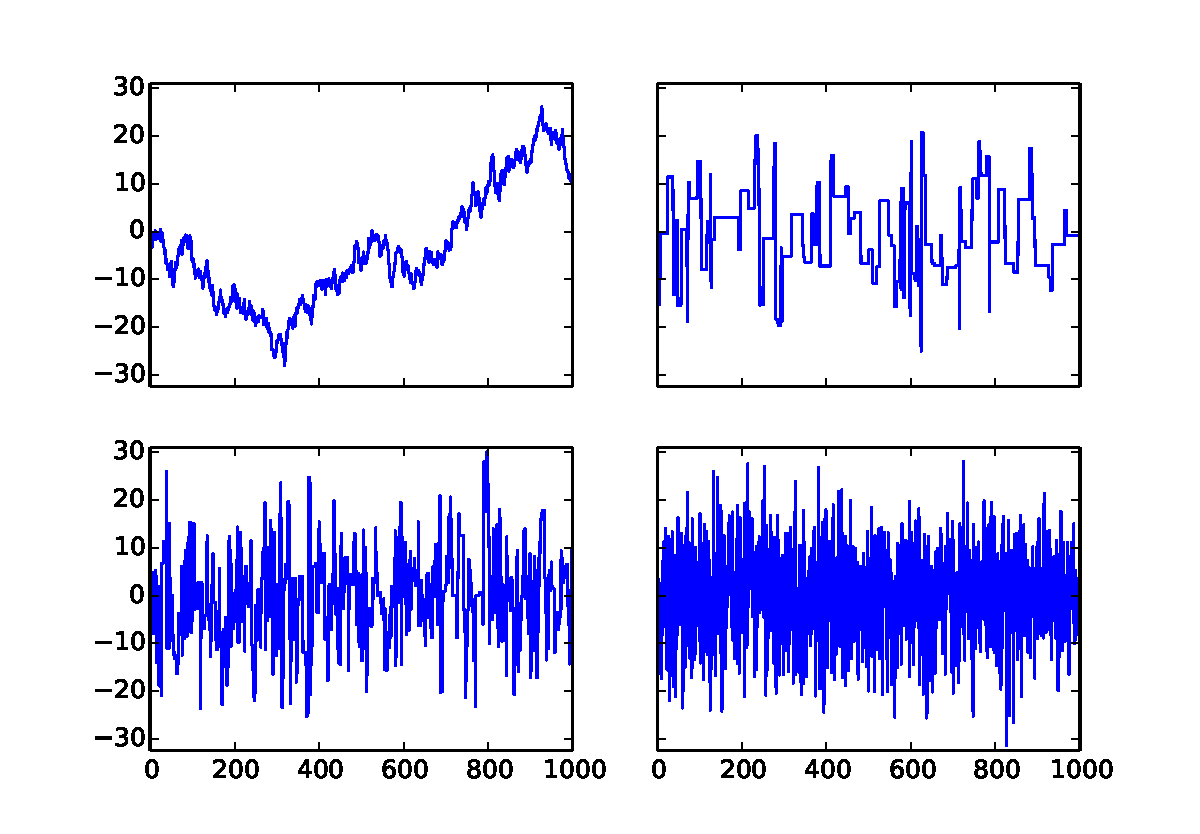
\includegraphics[width=\textwidth]{Figures/Acceptance_rates_high_low_optimal_iid.pdf}
\caption{\emph{Top}: Too high high (left, $0.96$) and too low (right, $0.13$) acceptance rates. \\\emph{Bottom}: approx. optimal rate for 1D target (left, $0.47$), i.i.d. target samples (right).}
\label{fig:acc_rates_high_low_opt}
\end{center}
\end{figure}

\subsection{Optimal scaling in Random Walk MH}
We consider $d$-dimensional target densities which are completely determined by the marginals, i.e. every component follows some density $\targd_c$ and is i.i.d.:
\begin{equation}
\label{eq:factortarget}
\targd(x_1, x_2, \dots, x_d) = \targd_c(x_1)\targd_c(x_2)\cdots\targd_c(x_d)
\end{equation}
A further assumption is that $\targd_c$ is smooth. Under these strong assumptions and for an increment distribution with isotropic covariance matrix $\DNorm(0,\scale^2I_d)$, \cite{Roberts1997} proved that the optimal acceptance rate is  exactly $0.234$ as $d \rightarrow \infty$. The derivation of the result proceeds along the following lines. Let $\scale = \sfact/\sqrt{d}$ where $\sfact> 0$. \cmt{FOLLOWING COPIED VERBATIM FROM ROSENTHAL -  Consult \cite{Roberts1997} for understanding!} \todo{Then as
$d \rightarrow \infty$, if time is speeded up by a factor of $d$, and space is shrunk by a factor of $\sqrt{d}$, then each component of the Markov chain converges to a diffusion having stationary distribution $\targd_c$, and speed function given by $\speed(\sfact) = 2\sfact^2\DNormCDF(-0.5\sqrt{I}\sf	act)$. Here $\DNormCDF$ is the CDF of the standard normal distribution, and $I$ is a constant given by $I = \Expect_{\targd_c}\left[  \left(\frac{\targd'_c(X)}{\targd_c(X)} \right)^2 \right] $}. Then by maximizing speed, the diffusion is optimal by all of the criteria given in \ref{sec:criteria_mcmc}:
$$\sfact_\textrm{opt} = \textrm{arg~max}_\sfact \speed(\sfact)$$
Nummerically, \cite{Roberts1997} found $\sfact_\textrm{opt} = 2.38/\sqrt{I}$ \todo{did \cite{Roberts1997} really state that? check!}, and as they also derived the asymptotic acceptance rate as $2\DNormCDF(-0.5\sqrt{I}\sfact)$, we can just plug in $\sfact_\textrm{opt}$ to get the optimal acceptance rate $A_\textrm{opt}$ (again, under the strong assumptions above and asymptotically for $d \rightarrow \infty$) as  $$A_\textrm{opt} = 2\DNormCDF(-0.5\sqrt{I}~\sfact_\textrm{opt}) = 0.234$$.
\todo{More results for more general cases, all leading to about $A_{opt} =0.234$ with some exceptions}

\subsection{Optimal scaling in MALA}
The Metropolis Adjusted Langevin Algorithm (MALA) \cite{Roberts1996} is similar to random walk MH with the difference that the random increments to the state of the Markov Chain are not centered on $0$. Rather, the increments at a given current state $\smp_n$ are distributed as $\DNorm(\frac{\scale^2}{2}\nabla \textrm{log}~\targd(\smp_n),\scale^2I_d)$ (see \ref{sec:lmc} for an overview of MALA and its truncated variant MALTA). In this case, \cite{Roberts1998} proved that under the assumption \eqref{eq:factortarget} and $\scale = \sfact/\sqrt[6]{d}$, we get 
 $$A^\textrm{MALA}_\textrm{opt} =  0.574$$
 The optimal scaling $\scale$ is bigger than in the random walk case \todo{check in original \cite{Roberts1996}}. 
 \begin{figure}[htbp]
\begin{center}
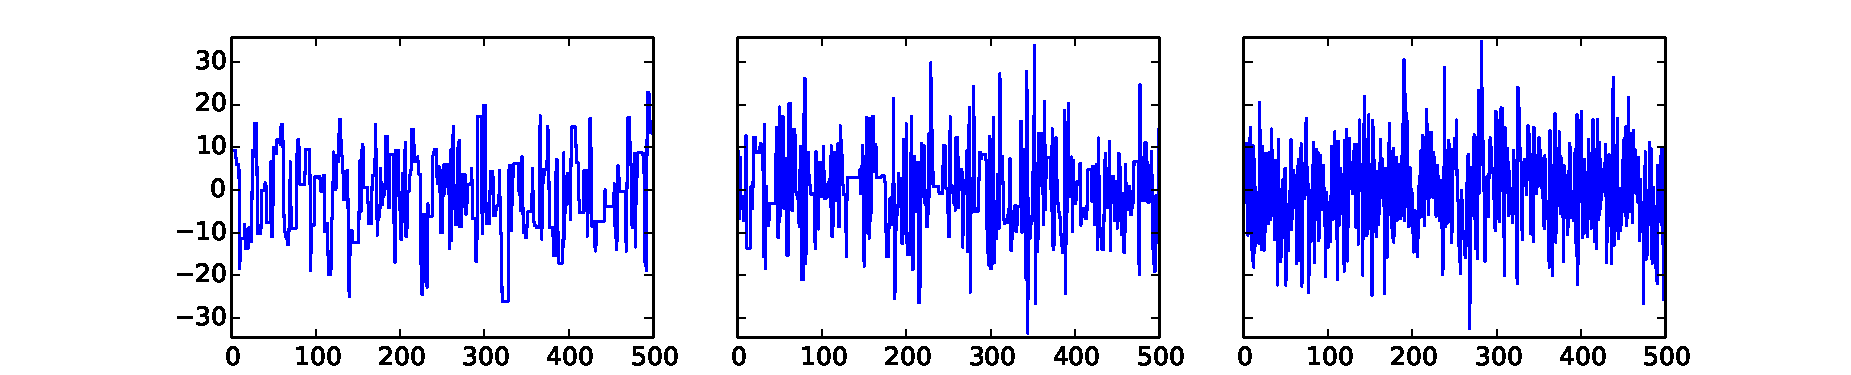
\includegraphics[width=\textwidth]{Figures/RW_vs_MALA_vs_iid.pdf}
\caption{Traces of state space of RW ($0.43$ left) and MALA ($0.58$ middle) with chains tuned for optimal acceptance rate, i.i.d. samples (right) for comparison}
\label{fig:rw_vs_mala}
\end{center}
\end{figure}

\subsection{Adaptivity}
When optimal acceptance rates are known, the experimenter might just run the MCMC algorithm and tune $\scale$ to get close to $A_\textrm{opt}$. This of course is tedious as it requires human intervention. While this can be automated in a straight forward way, tuning a single scale parameter might not be the only type of adaptivity that makes sense. The following section will thus look at the general case of algorithms that aim at automatically improving the sampling procedure while still ensuring ergodicity with respect to the target density.

\section{Automatic adaptation and ergodicity of sampling algorithms}
In the following, we will take a closer look at \emph{adaptive MCMC} algorithms and under which conditions they are ergodic with respect to some target density. Traditional Markov Chain Monte Carlo algorithms assume that the transition from state $\smp_n$ to state $\smp_{n+1}$ is markovian (i.e. can be described by a Markov Kernel $\MK(\cdot, \smp_n)$, hence \emph{Markov Chain}). Confusingly, adaptive MCMC algorithms do not necessarily construct a Markov Chain with respect to $\smp$. For many algorithms, the process $\{\smp_n,\MK_n\}_{n=0}^\infty$ (where $\MK_n$ is the kernel used at iteration $n$) is Markovian, but not even this is a necessary condition. A more appropriate name would thus be something along the lines of \emph{adaptive ergodic Monte Carlo}.\\
In the following, we use a set of Markov Kernels $\{\MK_i\}_{i \in \mathcal{I}}$, all of which have $\targd$ as their unique stationary distribution. At the $n$th iteration, we denote by $\MK_n$ the Kernel that is used to generate a new sample. One might expect that, as every $\MK_i$ has $\targd$ as stationary distribution, any mixture of the kernels in $\{\MK_i\}_{i \in \mathcal{I}}$ has the same property. However, \cite{Rosenthal2011} provides a simple counter example. Let $f$ be a probability mass function that is nonzero for each element of $\StateSp=\{1,2,3,4\}$

\begin{center}
\begin{tabular}{c|c c c c}
$x$ & $1$ & $2$ & $3$ & $4$\\
\hline 
$\targd(x)$ & $0.333$ & $0.001$ & $0.333$ & $0.333$
\end{tabular}
\end{center}

and $\targd(x) = 0$ for $x \notin \StateSp$. Now let $\MK'$ be a Metropolis-Hastings kernel with proposal $\propd(\cdot | \smp_n) = \textrm{Uniform}\{ \smp_n -1,  \smp_n+1\}$ and $\MK''$ one with proposal $\propd(\cdot | \smp_n) = \textrm{Uniform}\{\smp_n -2, \smp_n -1,  \smp_n+1, \smp_n +2\}$. Then because of the MH correction, both $\MK'$ and $\MK''$ are reversible and thus ergodic with respect to $\targd$. Now consider the following algorithm for adaptivity: set $\MK_{n+1} = \MK''$ if the $n$th move was accepted, $\MK_{n+1} = \MK'$ else. Now the adaptive algorithm can get stuck with using $\MK'$ in the state $\smp=1$ for many consecutive proposals and only has a probability of $0.001/0.333$ to switch to the usage of $\MK''$. Thus, informally, the adaptive mixture of ergodic (wrt $\targd$) kernels results in a sampling procedure that will yield state $1$ way more often than the equally probable states $3,4$.

Thus, we need to establish sufficient conditions for ensuring that adaptive MCMC algorithms preserve ergodicity. To this end, \cite{Roberts2007} provided results for a broad class of algorithms under rather weak assumptions. If the assumptions hold, asymptotic convergence (in the number of samples) of the sample approximation to the target $\targd$ holds, i.e.
\begin{equation}
\lim_{n \rightarrow \infty} \sup_{A\subseteq \StateSp} \|P(\smp_n \in A) - \targd(A)\| = 0
\end{equation}
 and furthermore a weak law of large numbers, i.e.
 \begin{equation}
\lim_{n \rightarrow \infty} \sum_{i=1}^n \targfunc(\smp_i) = \targd(\targfunc)
\end{equation}
for all bounded integrands $\targfunc: \StateSp \rightarrow \mathbb{R}$. The assumptions are  \emph{Diminishing Adaptation}
\begin{equation}
\label{eq:dimin_adapt}
\lim_{n \rightarrow \infty} \sup_{x \in \StateSp} \|\MK_{n+1}(x, \cdot) - \MK_{n}(x, \cdot)\| = 0 \textrm{ in probability}
\end{equation} 
and \emph{Bounded Convergence} (or \emph{Containment})
\begin{equation}
\label{eq:bound_conv}
\{M_\epsilon(\smp_n, n)\}_{n=0}^\infty \textrm{ is bounded in probability}
\end{equation} 
where $M_\epsilon(x, n) = \inf\{\|\MK_n^i(x, \cdot) - \targd(\cdot) \| \leq \epsilon : i \geq 1 \}$ for some $\epsilon > 0$ is called the $\epsilon$ convergence time for kernel $\MK_n$ when starting from state $x$. Assumption \eqref{eq:dimin_adapt} is the stronger of the two. In English, it says that the amount of adaptation goes to $0$ for growing $n$. An important note here is that there can still be an infinite total amount of adaptation (as the assumption is not  $\sum_{n=1}^\infty \sup_{x \in \StateSp} \|\MK_{n+1}(x, \cdot) - \MK_{n}(x, \cdot)\|< \infty$). Also, the limit $ \lim_{n \rightarrow \infty} \MK_n$ does not need to exist, i.e. the sequence of used Markov Kernels does not have to converge to some fixed kernel. One way of ensuring \eqref{eq:dimin_adapt} is to adapt at iteration $n$ with some probability $p(n)$ and have $\lim_{n \rightarrow \infty} p(n) = 0$. Also, in the case where $\MK_n$ uses an average of the previous $n$ samples, then as the new sample only contributes $\frac{1}{n}$th to the average, the amount of adaptation goes to $0$ for growing $n$.\\
Assumption \eqref{eq:bound_conv} on the other hand holds when $\StateSp \times S_\MK$ is finite (where $S_\MK$ is the set of used Markov Kernels), or compact in a topology where the kernels in $S_\MK$ or the Metropolis-Hastings proposal densities $\{\propd_n\}_{n=1}^\infty$ have a jointly continuous density \citep{Rosenthal2011,Roberts2007}. It basically says that for any combination of current sample $\smp$ and chosen kernel $\MK$, iteratively applying $\MK$ will ensure that the sampling approximation is less than $\epsilon$ away from target $\targd$ in a finite number of iterations. Thus, this condition is often easily satisfied \citep[though counterexamples can be constructed, see ][]{Rosenthal2011}.\\
In the following I will introduce some of the adaptive MCMC algorithms from the literature. The first important modern algorithm is the Adaptive Metropolis algorithm of \cite{Haario2001}.

\subsection{Adaptive Metropolis}
The first representative algorithm in the class of adaptive MCMC, the Adaptive Metropolis (AM) Algorithm \cite{Haario2001}, fits a Gaussian approximation with mean $\bar{\smp}_{n}$ and covariance matrix $C_n$ to the samples acquired up until iteration $n$. This is achieved by the recursion formula
\begin{equation}
\label{eq:haario_cov}
C_n = \begin{cases}
C_0 & n \leq n_0 \\
\scale_d (cov(X_0,\dots, X_{n-1}) + \epsilon I)& n > n_0
\end{cases}
\end{equation}
For an initial $C_0$ and some $n_0$ and where $\scale_d>0$ and $\epsilon>0$ are tunable parameters. Adding $\epsilon$ to the diagonal ensures that $C_n$ does not degenerate to zero. To update $C_n$ with a new sample $X_n$, we can use a recursion formula 
\begin{equation*}
C_{n+1} = \frac{n-1}{n} C_n + \frac{\scale_d}{n} \left (n\bar{X}_{n-1}\bar{X}^T_{n-1} - (n+1) \bar{X}_{n}\bar{X}^T_{n} + {X}_{n}{X}^T_{n}  + \epsilon I\right )
\end{equation*}
The proposal distribution for a new point given the last sample is $\smp_n$ then is
\begin{equation}
\label{eq:am_prop_orig}
q_\textrm{AM}(\cdot|\smp_n) = \DNorm(\smp_n, C_n)
\end{equation}
and a value $\smp^*$ is accepted with probability $min(1,\targd(\smp^*)/\targd(\smp_n))$. \cite{Haario2001} suggested that $\scale_d$ will be set depending only on the dimensionality of the domain of $\targd$. In the case where $\targd$ can be approximated by a gaussian, \cite{Rosenthal2011}  suggest to use $\scale_d = 2.38^2/d$. A minor variant of the AM algorithm is given in \cite{Roberts2009}. Instead of adding $\epsilon$ to the diagonal, they propose using a mixture proposal
\begin{equation}
\label{eq:am_prop_mod}
q'_\textrm{AM}(\cdot|\smp_n)  = (1-\beta)\DNorm(\smp_n, \scale_d~cov(X_0,\dots, X_{n-1}) ) + \beta \DNorm(\smp_n, \Sigma)
\end{equation}
 for a $\beta \in (0,1)$ and some fixed covariance matrix $\Sigma$.
 
 Since the adaptation at the $n$th step decreases as $\BigO(\frac{1}{n})$, the diminishing adaptation assumption \eqref{eq:dimin_adapt} is satisfied. The bounded convergence conditon \eqref{eq:bound_conv} holds if the target density $\targd$ decays at least polynomially in each coordinate, thus ensuring that the entries of the fitted covariance matrix will stay finite and actually converge to some fixed value. In conclusion, AM is ergodic with respect to $\targd$. The literature \citep{Haario2001,Roberts2009} and my own experiments in section \ref{sec:eval} suggest that AM is a very robust algorithm even for very high dimensions and outperforms non-adaptive sampling algorithms using gradient information such as Hamiltonian Monte Carlo \citep{Neal2011} tuned for optimal acceptance rate. The main problem AM poses is a computational one. In high dimensions, computing a matrix inverse or Cholesky factorization of the empirical covariance matrix after one new sample is acquired is prohibitively slow. One way to ameliorate this problem is to only adapt every $k$ iterations (and take all $k$ new samples into account). Another is to directly update the empirical covariance in its Cholesky form \citep[see e.g. ][]{Rasmussen2006}. In this case, the proposal in \eqref{eq:am_prop_mod} is the natural choice, as it is not  clear whether rank one updates are possible if some $\epsilon$ is added to the diagonal of the empirical covariance. However, updating the eigendecomposition of the empirical covariance one might still be able to use of the proposal distribution \eqref{eq:am_prop_orig}\footnote{Personal communication with Yee Whye Teh}.

\subsection{Adaptive MALTA}
An algorithm similar to AM making use of gradient information is the adaptive Metropolis Adjusted Langevin Algorithm with truncated drift \citep[adapt. MALTA, ][]{Atchade2006}. It uses parameters $0 < \epsilon_1 <A_1, \epsilon_2 >0$ and $\gamma_n$ which depends on the iteration index. To the process $(\smp_n)$ on the sample space $\StateSp$ adaptive MALTA adds an adaptation process $(\mu_n, \Gamma_n, \scale_n)$ on a space denoted $\Theta$. To give an intuition, $\mu_n$ will be (close to) a fit of the empirical mean of $(\smp_n)$, $\Gamma_n$ will be close to the empirical covariance of $(\smp_n)$ and the parameter $\scale_n$ is a scale parameter, similar to the parameter of the same name in AM. Let $C_n = \scale^2_n(\Gamma_n+\epsilon_2 I)$ for some parameter $\epsilon_2$. When the last sample is $\smp_n$, adaptive MALTA uses a proposal distribution
$$\propd(\cdot| \smp_n) = \DNorm(\smp_{n} + \frac{C_n}{2} D(n, \smp_{n}), C_n)$$
and a proposed move to $\smp^*$ is accepted with the standard MH probability
$$p_n^\textrm{acc}(\smp^*|\smp_n) = \textrm{min}\left(1, \frac{\targd(\smp^*)q(\smp_n|\smp^*)}{\targd(\smp_n)q(\smp^*|\smp_n)} \right)$$
The subscript $n$ hints at the fact that the acceptance probability depends on the parameter values at time $n$ through $\propd$.
 $D(\cdot, \cdot)$ is a drift function and \cite{Atchade2006} suggests
$$D(k, x) = \frac{\delta}{\textrm{max}(\delta, |\nabla~\textrm{log}~\targd(x)|)}\nabla~\textrm{log}~\targd(x)|$$
The scale parameter is constrained to the interval $[\epsilon_1,A_1]$ by the projection
\begin{equation*}
p_1(\scale) = 
\begin{cases}
\epsilon_1 & \scale <\epsilon_1 \\
A_1 & \scale > A_1 \\
\scale & \textrm{else}
 \end{cases}
 \end{equation*}
The covariance $\Gamma_n$ is constrained to lie in the convex compact cone defined by the projection
\begin{equation*}
p_2(\Gamma) = \begin{cases}\Gamma &|\Gamma| \leq A_1 \\ 
 \frac{A_1}{|\Gamma|}\Gamma &\textrm{else}
 \end{cases}
 \end{equation*}
where $|\cdot|$ is the Frobenius norm. Finally, $\mu_n$ is constrained to the ball $B(0,A_1)$ in $\mathbb{R}^d$ (where $d$ is the dimensionality of the problem) by the projection
\begin{equation*}
p_3(\mu) = \begin{cases}A_1 &|\mu| \leq A_1 \\ 
 \mu &\textrm{else}
 \end{cases}
 \end{equation*}
 Suppose we have generated a new sample $\smp_{n+1}$. Now the parameters are adapted using the following equations.
\begin{eqnarray*}
\mu_{n+1} &= &p_3(\mu_n+\gamma_n(\smp_{n+1} -\mu_n))\\
\Gamma_{n+1} &=& p_2(\Gamma_n + \gamma_n((\smp_{n+1}-\mu_n)(\smp_{n+1}-\mu_n)^T-\Gamma_n)\\
\scale_{n+1} &= &p_1(\scale_n+\gamma_n(p_n^\textrm{acc}(\smp^*|\smp_n)-\tau))
\end{eqnarray*}
Where $\tau$ is the optimal acceptance rate that the algorithm should try to attain and $\gamma_n$ is a factor decreasing the amount of adaptation for each new sample. Concretely,  $\lim_{n \rightarrow \infty}\gamma_n = 0$ and \cite{Atchade2006} used $\gamma_n = 10/n$. The values for the other parameters where set as $\epsilon_1 = 10^{-7}, \epsilon_2 = 10^{-6}, A_1=10^7$. 

As is evident even from this concise exposition to adaptive MALTA, it is a complex algorithm with many parameters (even though according to \cite{Atchade2006} the algorithm is not very sensitive to $\epsilon_1,\epsilon_2$ and $A_1$, so they might be considered fixed). Of course it has the advantage of working correctly even if the expectation or variance of $\targd$ does not exist. However, even when tuned to optimal acceptance rates, I found the performance of adaptive MALTA to often be worse than that of AM.



\section{Introduction: Gradient Importance Sampling}

Monte Carlo methods have been developed into one of the mainstream inference methods of Bayesian Statistics and Machine Learning over the last thirty years \cite{Robert2004}. They can be used to approximate expextations with respect to posterior distributions of a Bayesian Model given data. The most widely used Monte Carlo Method for this purpose today is Markov Chain Monte Carlo (MCMC). In this approach, a Markov Chain is constructed which is ergodic with respect to the given posterior distribution.
In parallel, a scheme for sampling from a sequence of target distributions, called Sequential Monte Carlo (SMC), has been developed \cite{Doucet2001a}. SMC has traditionally been used for inference in time series models and for online tracking applications. However, there has been a considerable amount of research on using SMC for inference in static models as well \cite{Chopin2002,DelMoral2006,Schafer2013}. In this paper, I will develop a powerful variant of SMC for static models making use of gradient information, dubbed Gradient Importance Sampling.

The paper will proceed as follows. In subsection \ref{sec:lmc} I will give a short overview of the a simple well-known MCMC algorithm making use of gradient information, the Metropolis Adjusted Langevin Truncated Algorithm. In subsection \ref{sec:ismc} an exposition to Importance Sampling and SMC is given. Gradient IS and its variants  are introduced in \ref{sec:GRIS}. Related work, especially in adaptive MCMC and Importance Sampling, is discussed in Section \ref{sec:relwork}. Gradient IS is evaluated and compared against previous algorithms in Section \ref{sec:eval}. The last section concludes.




\section{Gradient IS}
\label{sec:GRIS}
Gradient IS (GRIS) is a variant of Sequential Monte Carlo \cite{Doucet2001a}, or, when targeting the same density at each iteration, of its special case Population Monte Carlo \cite{Cappe2004}. GRIS accomplishes adaptivity by  fitting a covariance matrix $C_t$ to samples from the target density that have been gathered at time $t$. The proposal distribution for a new sample given an old sample $\smp'$   is then given by
\begin{equation*}
q_{t}(\cdot | \smp' ) = N(\cdot | \smp'  + D(t, \nabla~\textrm{log}~f(\smp' )), C_t)
\end{equation*}
 where $D$ is a drift function. We used $$D(t,  \nabla~\textrm{log}~f(\smp' )) = (\delta /t^{1.5})  \nabla~\textrm{log}~f(\smp' )$$ thus introducing a parameter $\delta \geq 0$ (and usually $\delta \leq 1$) which ought to be tuned for each target density. 
To fit $C_t$ we use the parametrization \todo{How strongly does this overlap with the section on Adaptive Metropolis in the adaptive MCMC part?}
\begin{equation*}
C_t = \begin{cases}
C_0 & t \leq t_0 \\
s_d (cov(X_0,\dots, X_{t-1}) + \epsilon I)& t > t_0
\end{cases}
\end{equation*}
For an initial $C_0$ and some $t_0$ and where $s_d>0$ and $\epsilon>0$ are tunable parameters. To update $C_t$ with a new sample $X_t$, we can a recursion formula 
\begin{equation*}
C_{t+1} = \frac{t-1}{t} C_t + \frac{s_d}{t} \left (t\bar{X}_{t-1}\bar{X}^T_{t-1} - (t+1) \bar{X}_{t}\bar{X}^T_{t} + {X}_{t}{X}^T_{t}  + \epsilon I\right )
\end{equation*}
Where $\bar{X}_t$ is the running average at iteration $t$ (with an obvious recursion formula) \cite{Haario2001}.
Directly updating either the Cholesky or Eigendecomposition of $C_t$ results in significant computational savings, especially when the updates are done frequently. Both decompositions can be used to draw samples from and evaluate the density of the respective multivariate normal, both of which are prerequisites of the GRIS algorithm. A complementary method to tradeoff speed and adaptivity is to collect more than one new sample before updating. GRIS then proceeds as given in  Algorithm~\ref{algo:lis}.

\begin{algorithm}[tb]

\caption{Gradient IS algorithm}
\begin{algorithmic}
\label{algo:lis}
   \STATE {\bfseries Input:} unnormalized density $f$, gradient $\nabla~\textrm{log}~f$, population size $p$, $p$ intial samples $S$, sample size $m$
    \STATE {\bfseries Output:} list $S$ of $m$ samples
   \WHILE{$len(S) < m + p$}
   	\STATE Initialize $P = List()$
	\STATE Initialize $W = List()$
	%%
	\FOR{$i=1$ {\bfseries to} $p$}
		\STATE (a) sample $\smp' $ uniformly from last $p$ samples in $S$
		\STATE (b) generate $\smp \sim q_{t}(\cdot | \smp' )$, append it to $P$
		\STATE ~~~append weight $f(\smp)/q_{t}(\smp)$ to $W$
   	\ENDFOR
	\STATE resample $p$ values from $P$ with repl. according 
	\STATE ~~~to weights and append samples to $S$
	\STATE compute $C_{t+1}$
	%%

   \ENDWHILE

   \STATE remove first $p$ samples from $S$
\end{algorithmic}

\end{algorithm}

\subsection{Gradient IS with a sequence of target distributions}
\label{sec:seqin}
Instead of using the correct target distribution $f$ at every IS iteration like in PMC, it is also possible to construct a sequence of intermediate target distributions $(g_t)_{t=1}^T$ where $g_T = f$. In the existing SMC literature addressing static targets, only the samples acquired when targeting the actual distribution of interest are then used for estimating the integral $H$ \cite{DelMoral2006,Schafer2013}. This approach is very robust when compared to MCMC algorithms, as it explores the probability space better \cite{Schafer2013,Chopin2002}.\\
One possibility for constructing a sequence of distributions is the geometric bridge defined by $g_t \propto g_0^{1-\rho_t} f^{\rho_t}$  for some initial distribution $g_0$ and where $(\rho_t)_{t=1}^T$ is an increasing sequence satisfying $\rho_T = 1$. Another is to use a mixture $g_t \propto ({1-\rho_t})g_0+ {\rho_t}f$. When $f$ is a Bayesian posterior, one can also add more data with increasing $t$, e.g. by defining the intermediate distributions as $g_t(\smp) = f(\smp|d_1,\dots,d_{\floor{\rho_t D}})$ where $D$ is the number of data points, resulting in an online inference algorithm \cite{Chopin2002}.

However, when using a distribution sequence that computes the posterior density $f$ using the full dataset (such as the geometric bridge or the mixture sequence), one can reuse the intermediate samples when targeting $g_t$ for posterior estimation using a simple trick. As the value of $f$ is computed anyway for the harmonic bridge and the mixture sequence, we can just use the weight $f(\smp)/q_t(\smp)$ for posterior estimation while employing $g_t(\smp)/q_t(\smp)$ to inform future proposal distributions. This way the evaluation of $f$ (which is typically costly) is put to good use for improving the posterior estimate. To the best of my knowledge, this recycling of samples in SMC for static targets has not been reported in the literature.

\section{Related work}
\label{sec:relwork}

\subsection{Adaptive Monte Carlo using ergodic stochastic processes}

\todo{rewrite in light of the earlier section on adaptive MCMC}
Adaptive MCMC algorithms use samples acquired so far in order to tune parameters of the sampling algorithm to adapt it to the  target.  which is another difference from GRIS, which uses importance weighting instead. The AM algorithm is the first adaptive MCMC algorithm and is provably ergodic wrt the target distribution $f$.

Informally, adapting the Markov Kernels used in MCMC will result in an algorithm that is ergodic with respect to target $f$ in the general case as long as 
\begin{enumerate}
	\item all Markov kernels used are ergodic wrt target $f$ (have $f$ as their stationary distribution)
	\item adaptation diminishes, e.g. adaptation probability $p_t$ for iteration $t$ satisfies $p_t~\rightarrow~0$ as $t~\rightarrow~\infty$.
\end{enumerate}
(Theorem 1 in \cite{Roberts2007}). We can still have $\sum^N_{t=1}p_t {\rightarrow} \infty$ as $N\rightarrow\infty$, i.e. infinite overall adaptation (as in \cite{Sejdinovic2013}). It is important to note that the diminishing adaptation is sufficient but not necessary. Other schemes might still be ergodic, one example being the AM algorithm, where adaptation is not diminished.

\subsection{Adaptive Importance Sampling Schemes}

Adaptive Importance Sampling schemes in related to SMC have mostly been trying to fit a closed-form approximation to the posterior for usage as a proposal distribution in the next iteration. In particular, previous work used optimality criteria such as minimization of KL-divergence between proposal distribution and posterior to asses the quality of the proposal distribution. After collecting new samples, D-Kernel approximations \cite{Douc2007} or Mixture distributions (such as Mixtures of Gaussians or Student-T mixtures) \cite{Cappe2008} are updated to fit the posterior better.
In another line of research, better ways of using the produced samples have been sought. A particularly interesting approach is Adaptive Multiple Importance Sampling \cite{Cornuet2012,Marin2012}. Here, samples from previous proposal distributions are reweighted after the sampling is finished in order to reflect the overall proposal distribution used across iterations. This is achieved by simply assuming that each weighted sample is produced by a mixture over the proposal distributions used, where the mixture weight is proportional to the number of samples actually drawn from a particular proposal. This reweighting has been shown to be consistent and considerably improve consecutive estimates \cite{Marin2012}.

\section{Evaluation}
\label{sec:eval}
For an experimental evaluation of the adaptive Gradient IS algorithm, I targeted three synthetic distributions (i.e. not posteriors based on some dataset) and one posterior of a Bayesian Logistic regression model. The synthetic distributions have the advantage that the expected value $H$ of the target is known in closed form, for the Logistic Regression dataset ground truth was estimated in a separate Monte Carlo experiment. I started the simulation at $H$ to avoid having to handle burn-in for MCMC and ran $20$ Monte Carlo simulations with $3000$ target or gradient evaluations each. If the target and its gradient are evaluated at the same point, this is counted as a single evaluation. This is justified by the fact that most of the time either likelihood or gradient calculation dominate complexity and computing the other value uses only little additional time (since factors common to both likelihood and gradient can be cached).  I compared to the AM algorithm, adaptive T-MALA, and Hamiltonian Monte Carlo \cite{Neal2011} MCMC algorithms, where I tuned the parameters to give optimal acceptance rates as reported in the literature. GRIS was tuned for low estimates of Monte Carlo variance, an information that is available in typical black-box situations (i.e. where nothing is known about the target $f$ except the information produced by the sampling algorithm). Is used the variant of GRIS that did not use a sequence of target distributions as it gave good results and was easier to implement.

\subsection{Maximum squared errors and Effective Sample Size}
Estimating  Effective Sample Size (ESS) is easy in traditional Importance Sampling and does not require establishing ground truth. Given importance weights of $N$ collected samples $(w_i)_{i=1}^N$ and their normalized version $\widehat{w}_i = w_i/\sum_{i=1}^N w_i$ we can compute ESS as 
$$\textrm{ESS}^\textrm{IS}_N = \frac{1}{\sum_{i=1}^N(\widehat{w}_i)^2} $$
If all the weights are the same (i.e. we have a sample coming from our target distribution), we have $\textrm{ESS}^\textrm{IS}_N = N$, whereas if only one of the weights is non-zero,  $\textrm{ESS}^\textrm{IS}_N = 1$. A necessary condition for this estimate to be valid however is that drawn importance samples are iid. For MCMC a similar estimate (under the same name) is available after establishing ground truth for an integral of interest. An exposition to this is given in \cite{Hoffman2014} whom we will follow. 
Given a function $\targfunc$ which we want to integrate wrt the target density $\targd$, and samples $\smp_1,\dots, \smp_N$ from a Markov Chain targeting $\targd$, that follow the distribution $\propd_{MC}$ we can use the estimate
$$\textrm{ESS}^\textrm{MC}_N = \frac{N}{1+2\sum_{i=1}^{N-1} (1-\frac{i}{N}) \acor_i^\targfunc} $$
where $\acor_i^\targfunc$ is the autocorrelation of $\targfunc$ under $\propd_{MC}$ at lag $i$.  If the autocorrelation is exactly  $0$ at each lag (i.e. all of the samples are independent), then again $\textrm{ESS}^\textrm{MC}_N=N$, as desired.  An estimate of autocorrelation is given by

$$\widehat{\acor}_i^\targfunc = \frac{1}{\Var[\targfunc(X)](N-i)} \sum_{j=i+1}^N (\targfunc(\smp_{j}) - \Expect[\targfunc(X)]) (\targfunc(\smp_{j-i}) - \Expect[\targfunc(X)])$$
In this autocorrellation estimate we make use of the ground truth values $\Expect[\targfunc(X)]$ and $\Var[\targfunc(X)]$ which can only be estimated by a long run of some Monte Carlo method when $\targd$ is a black block (for example when it is given only proportionally as a Bayesian posterior). Now as the estimate of autocorrelation is noisy for large lags, \cite{Hoffman2014} suggests to truncate the autocorrelations at the smallest cutoff $c$ with $\acor_c^\targfunc < 0.05$, yielding the estimator

$$\widehat{\textrm{ESS}}^\textrm{MC}_N = \frac{N}{1+2\sum_{i=1}^{c} (1-\frac{i}{N}) \widehat{\acor}_i^\targfunc} $$

Now as $\widehat{\textrm{ESS}}^\textrm{MC}$ is a univariate measure, \cite{Girolami2011,Hoffman2014} suggest the following approach: calculate ESS for each dimension separately and take the minimum across dimensions. Because usually in a bayesian setting one is interested in estimation of variance, the suggested procedure is to do this for an estimate of both expected value and variance of $\targd$ and take the minimum of those as the final ESS estimate.

Ironically, an ESS estimate does not exist for Sequential Monte Carlo when targeting the same density across iterations (the situation is different in a dynamic model with multiple targets). For one, it is not possible to use the estimate $\textrm{ESS}^\textrm{IS}$ because SMC induces dependency between samples. Also, $\textrm{ESS}^\textrm{MC}$ is not usable because the dependency structure in SMC, and thus the computation of autocorrelation, is much more complicated than in MCMC, as a sample at one iteration of the algorithm can spawn several samples in the next iteration.

However, using ground truth estimates $\Var[\targfunc(X)]$ and $\Expect[\targfunc(X)]$ as $\textrm{ESS}^\textrm{MC}$ does, it is possible to reproduce the worst case properties suggested by \cite{Girolami2011,Hoffman2014}. To this end, one measures maximum squared error (MaxSE) by computing, for each Monte Carlo run, squared errors with respect to $\Var[\targfunc(X)]$ and $\Expect[\targfunc(X)]$  and taking the maximum across those and across dimensions.


\subsection{Gaussian Grid}
The first target was a mixture of 25 2D Gaussians with equidistant means and mixture weights depending on distance from origin, a contour plot for which is given in Figure~\ref{fig:gauss_grid_contour}. A box plot for the squared error across different numbers of target evaluations is given in Figure~\ref{fig:gauss_grid_box}, where the box ranges from 1st to 3rd quartile and whiskers extend to $1.5*\textrm{IQR}$  (interquartile range). Hamiltonian Monte Carlo (HMC) was not plotted here, because the algorithm performed much worse than the other three candidates and proper scaling was impossible.

\begin{figure}[tbp]
\begin{center}
\begin{minipage}[t]{0.5\textwidth}
\centering
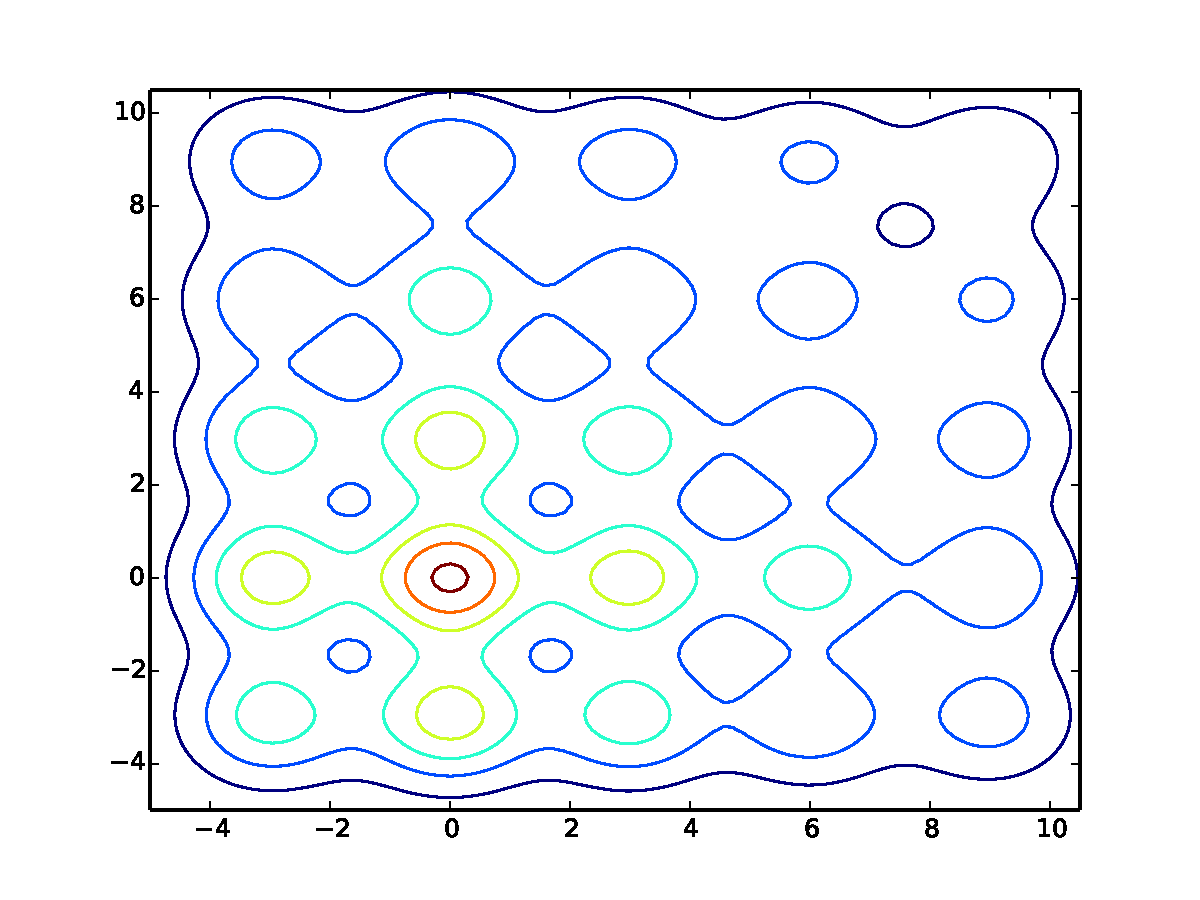
\includegraphics[width=0.8\textwidth]{figures/Gauss_Grid_Contour.pdf} 
\caption{Gaussian mixture target: Contour plot}
\label{fig:gauss_grid_contour}
\end{minipage}\hfill
\begin{minipage}[t]{0.5\textwidth}
\centering
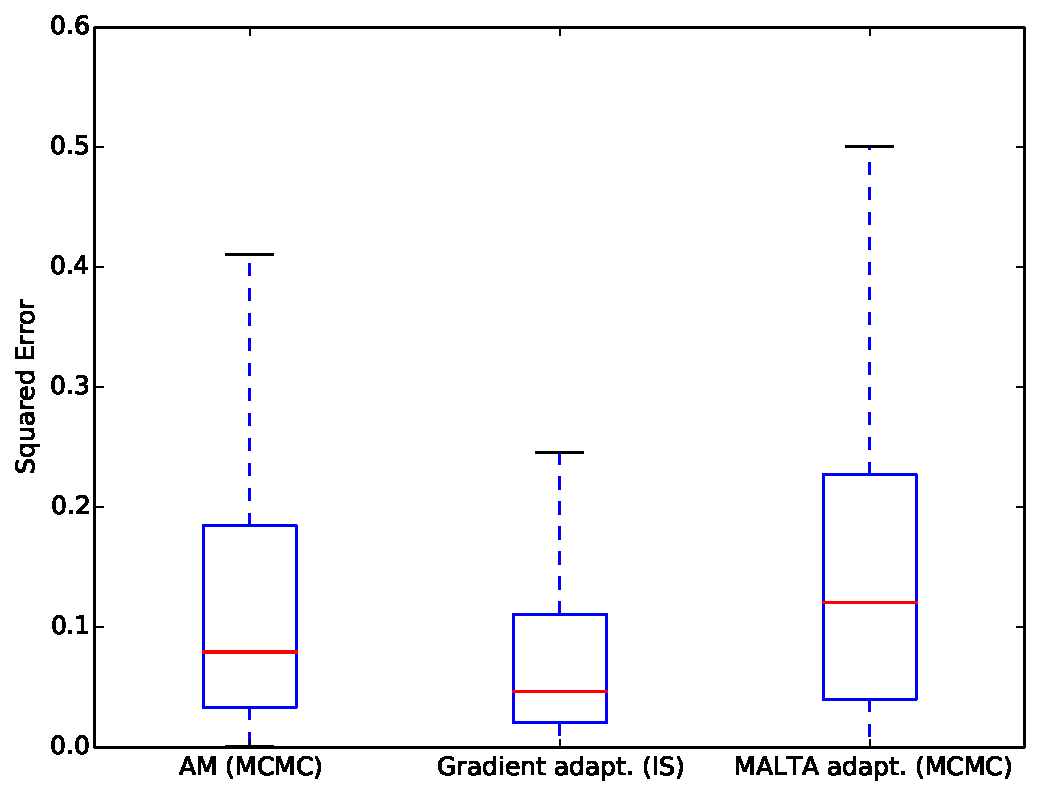
\includegraphics[width=0.9\textwidth]{figures/Gauss_Grid_boxplot.pdf} 
\caption{Gaussian Mixture target: SE performance. Algorithms not shown are widely off scale.} 

\label{fig:gauss_grid_box}
\end{minipage}

\end{center}
\end{figure}

For this target, the performance was very close for the adaptive algorithms. Adaptive Gradient IS exhibits smallest MSE and variance (see Figure~\ref{fig:gauss_grid_mse}), but the AM algorithm is a close second. As multimodal targets are traditionally problematic for gradient informed sampling algorithms, it is interesting to see that adapting to the posterior covariance structure of the target can help mitigate problems in this case. The particularly weak performance of HMC possibly stems from the algorithm getting stuck in different modes for different runs, explaining in particular the high variance (Figure~\ref{fig:gauss_grid_mse}). 



\begin{figure}[tbp]
\begin{center}
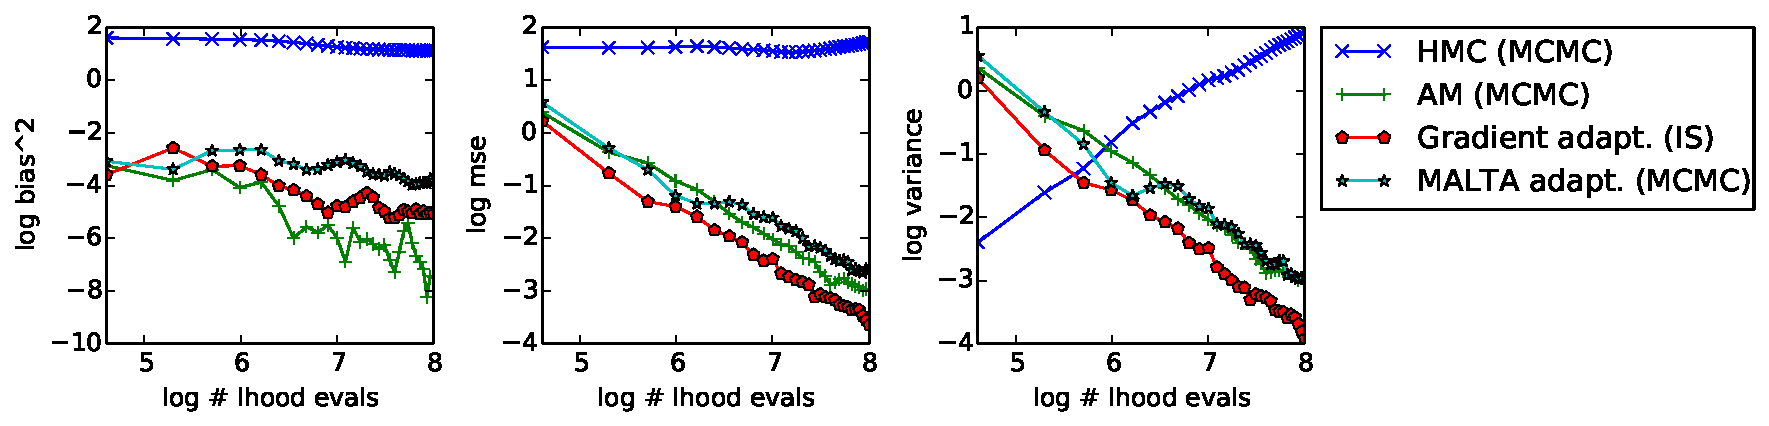
\includegraphics[width=0.8\textwidth]{figures/Gauss_Grid_b2_mse_var.pdf}
\caption{Gaussian mixture target: Squared bias, MSE and variance as a function of number of target evaluations}
\label{fig:gauss_grid_mse}
\end{center}
\end{figure}

\subsection{Banana}
The 2D Banana shaped unnormalized measure was given by $f(x) = \textrm{exp}(-\frac{1}{2s}x_1^2-\frac{1}{2}(x_2-b(x_1^2-s))^2$. The measure is determined by parameters $b$ and $v$ which where set to $100$ and $0.03$, respectively (see Figure~\ref{fig:banana_contour} for a contour plot). For unimodal targets, gradient based samplers are traditionally strong, though that advantage might be irrelevant when we adapt a scale matrix for a simple random walk algorithm. As is evident from Figures~\ref{fig:banana_box} and \ref{fig:Banana_mse}, the simple AM algorithm actually is competitive with adaptive T-MALA for this target. However, adaptive Gradient IS again shows gains here when compared to the other samplers. This is particularly encouraging since  T-MALA and Gradient IS are using the exact same drift function and T-MALA adapts more parameters than Gradient IS does. If the remaining parameters of Gradient IS can be adapted automatically, further improvements might be possible.

\begin{figure}[tbp]
\begin{center}
\begin{minipage}[t]{0.5\textwidth}
\centering
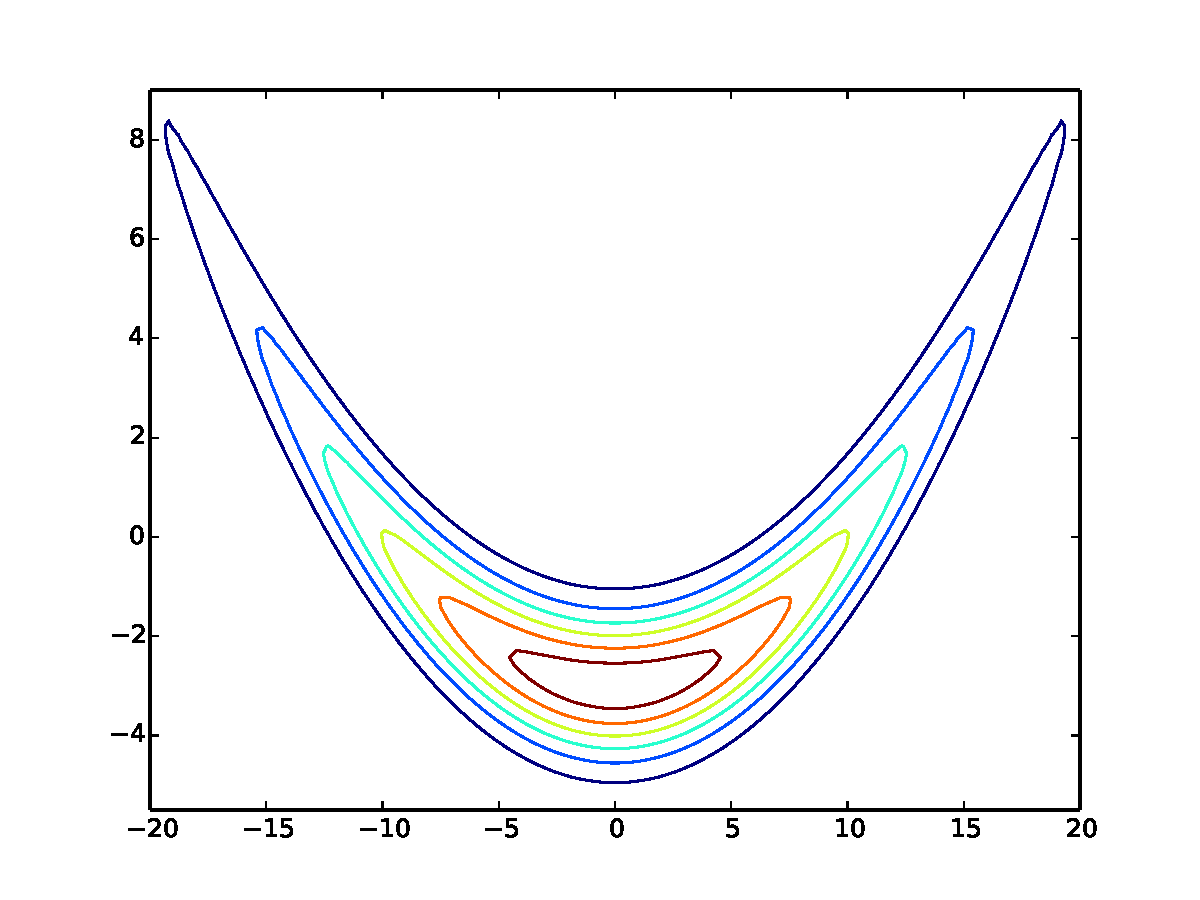
\includegraphics[width=\textwidth]{figures/Banana_Contour.pdf} 
\caption{Banana target: Contour plot}
\label{fig:banana_contour}
\end{minipage}\hfill
\begin{minipage}[t]{0.5\textwidth}
\centering
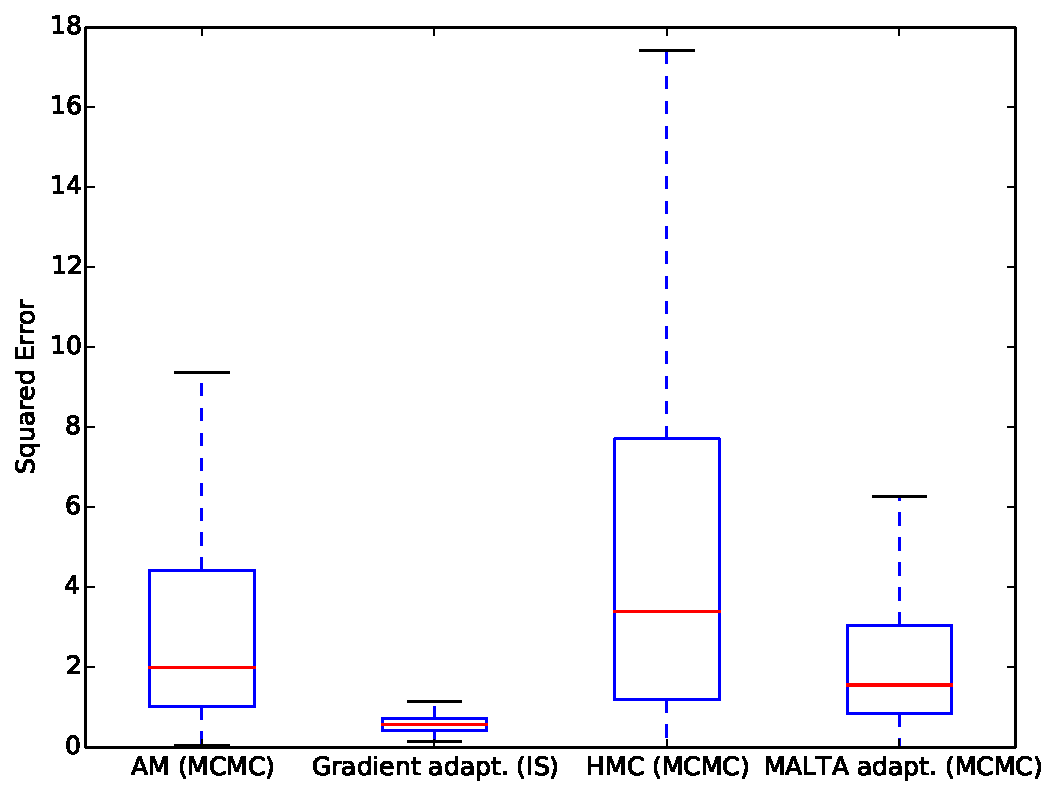
\includegraphics[width=\textwidth]{figures/Banana_boxplot.pdf} 
\caption{Banana target: SE performance} 

\label{fig:banana_box}
\end{minipage}

\end{center}
\end{figure}





\begin{figure}[tbp]
\begin{center}
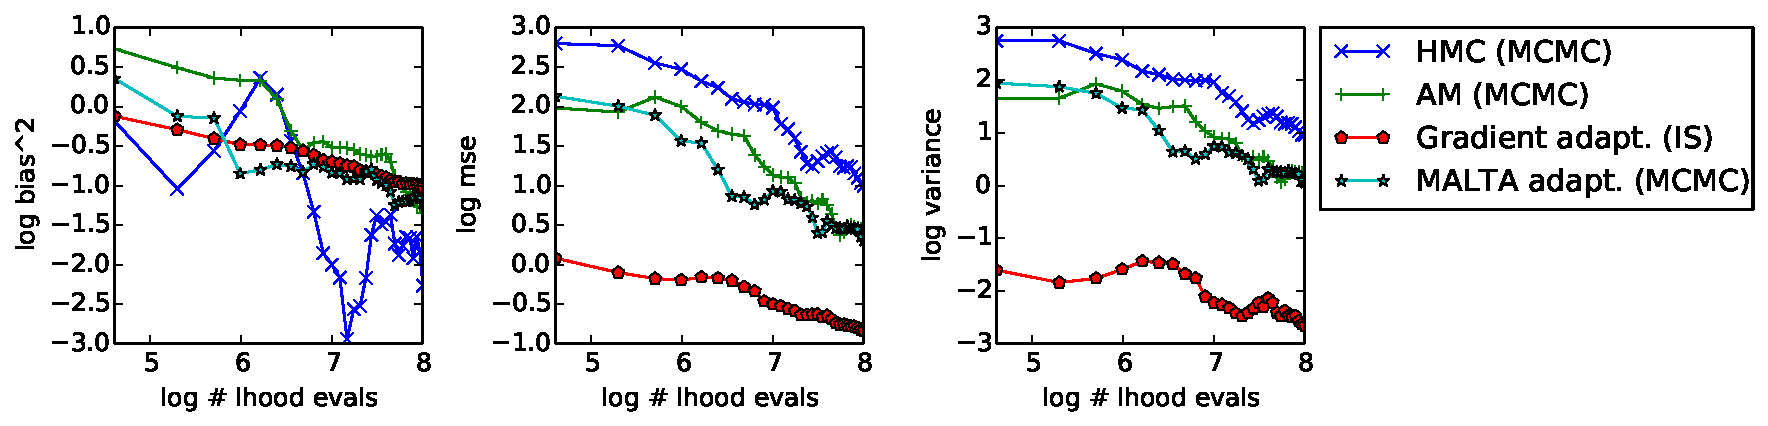
\includegraphics[width=0.8\textwidth]{figures/Banana_b2_mse_var.pdf}
\caption{Banana target: Squared bias, MSE and variance as a function of number of target evaluations}
\label{fig:Banana_mse}
\end{center}
\end{figure}

%\begin{figure}[tbp]
%\begin{center}
%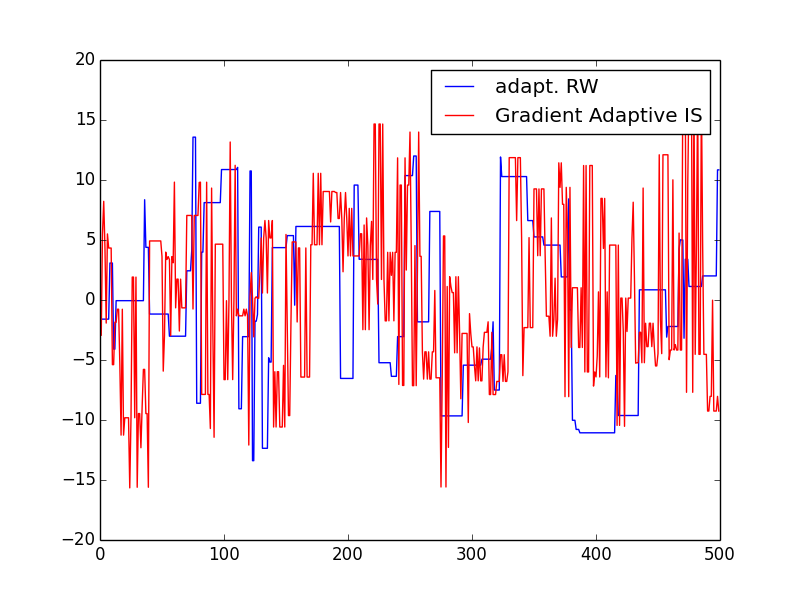
\includegraphics[width=0.5\textwidth]{figures/Banana_first_parameter_viz.png}
%\caption{Banana target: Location of first sample coordinate for last $500$ posterior samples}
%\label{fig:Banana_1d}
%\end{center}
%\end{figure}

\subsection{Mixture of T distributions}
The third target considered was a mixture of three $10$D multivariate $t$-distributions with different means, $10$ degrees of freedom and varying mixture weights. The scale matrices where drawn from an Inverse Wishart distribution with identity scale matrix and $10$ degrees of freedom, yielding mixture components with strong correlations among dimensions.  A contour of the marginal density of the last two coordinates is given in Figure~\ref{fig:t_mixt_contour}. This case was considered because $t$-distributions have heavier tails than Gaussians. As a standard rule of thumb, IS proposal distributions should have heavier tails than the target to ensure finite variance of the estimate \cite{Robert2004}. With a mixture of $t$-distributions, I wanted to experimentally check for any problems stemming from the Gaussian proposal used in all algorithms. GRIS is better when averaging squared error across dimensions (Figure \ref{fig:t_mixt_box}). Also, when when comparing maximum log squared errors GRIS is clearly an improvement over previous algorithms (Figure \ref{fig:t_mixt_mse}). 

\begin{figure}[tbp]
\begin{center}
\begin{minipage}[t]{0.5\textwidth}
\centering
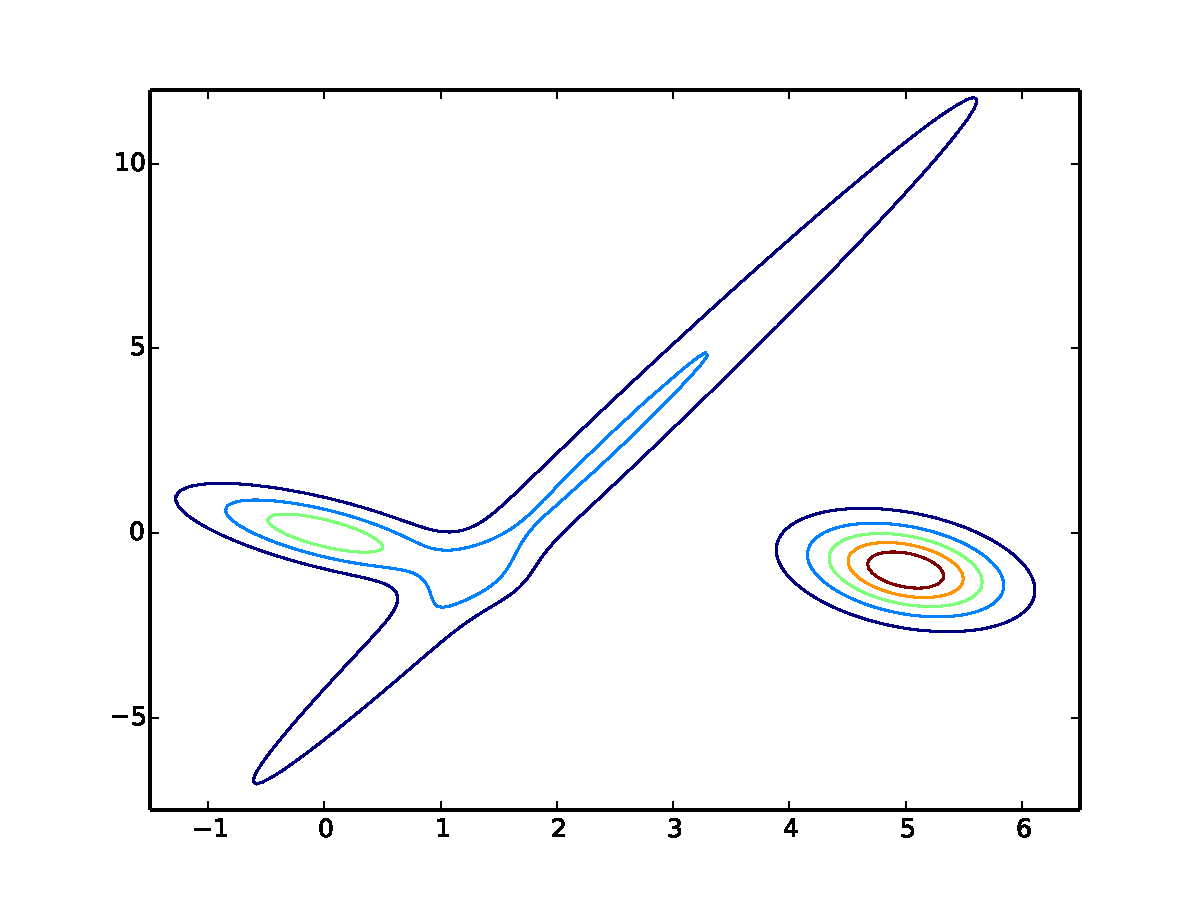
\includegraphics[width=\textwidth]{figures/T_Mixt_Contour.pdf} 
\caption{10 D $t$-Mixture target: Contour plot of the marginal density of the last two dimensions}
\label{fig:t_mixt_contour}
\end{minipage}\hfill
\begin{minipage}[t]{0.5\textwidth}
\centering
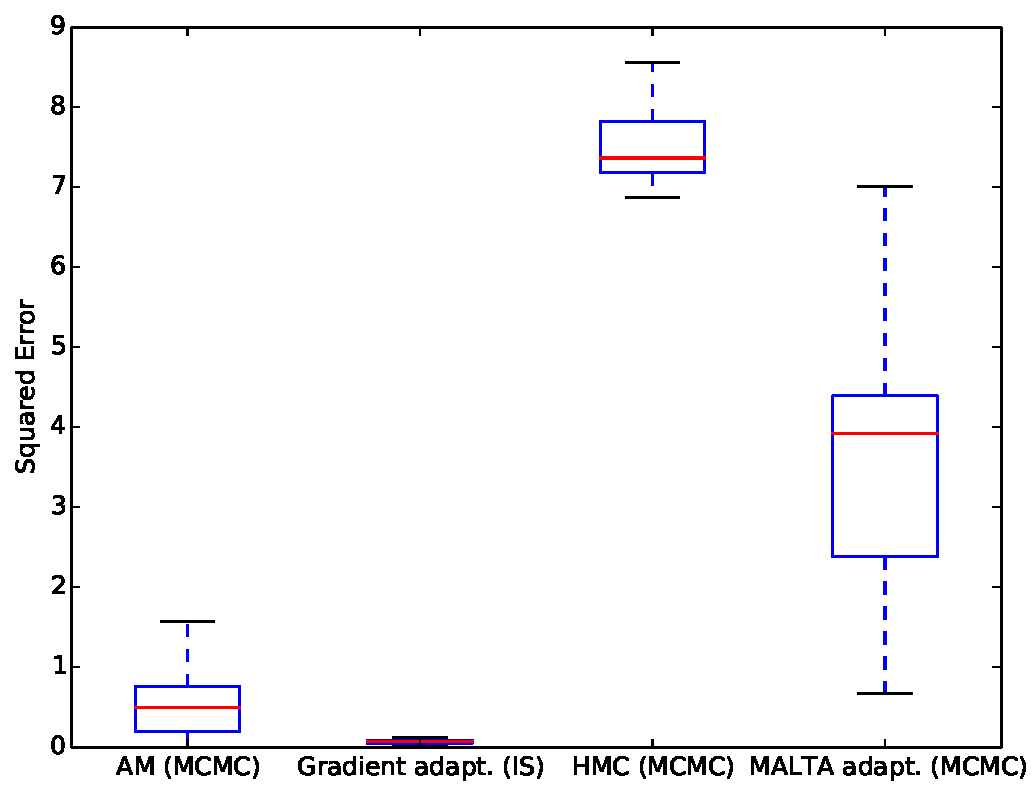
\includegraphics[width=0.8\textwidth]{figures/T_Mixt_boxplot.pdf} 
\caption{$t$-Mixture target: SE of mean estimates, averaged across dimensions} 

\label{fig:t_mixt_box}
\end{minipage}

\end{center}
\end{figure}



\begin{figure}[tbp]
\begin{center}
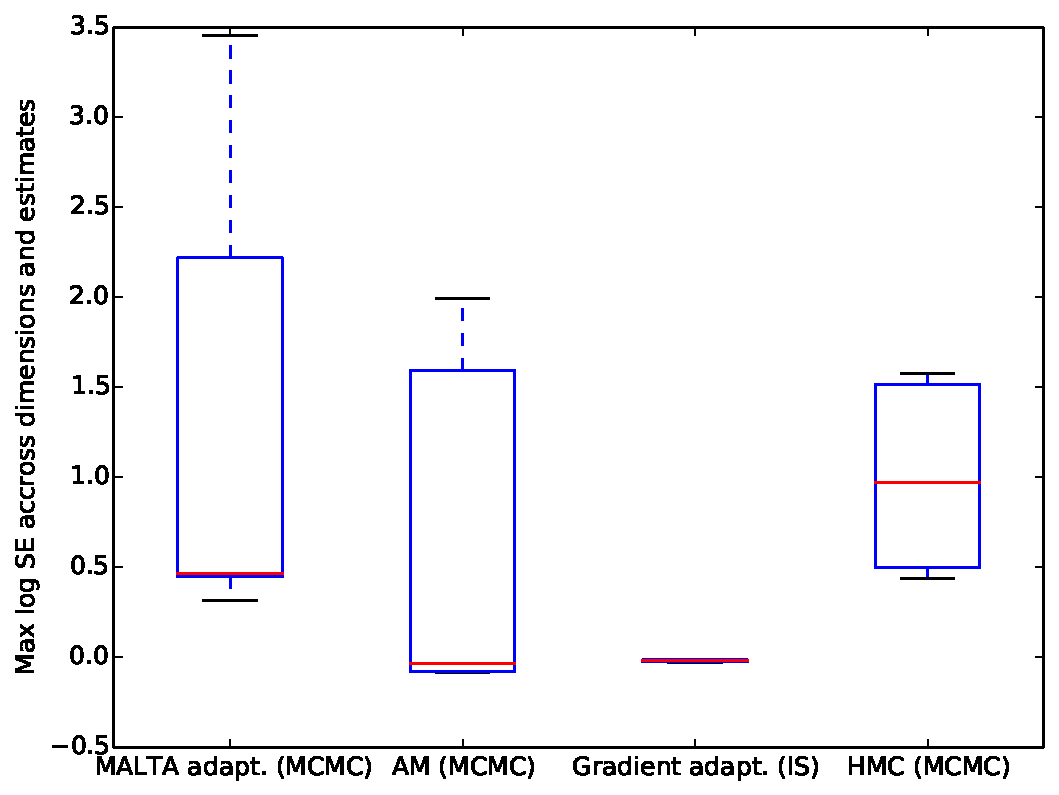
\includegraphics[width=0.5\textwidth]{figures/T_Mixture_worst.pdf}
\caption{$t$-Mixture target: Squared bias, MSE and variance as a function of number of target evaluations}
\label{fig:t_mixt_mse}
\end{center}
\end{figure}


\subsection{German Credit Dataset: Logistic regression}
The German Credit dataset was used with the Logistic Regression model developed in \cite{Hoffman2014}. This model exhibited a $25$D posterior distribution which allowed for a Laplace approximation. To find ground truth, I collected ordinary Importance Samples from a mixture between the Laplace Approximation and the sample approximation with slightly increased scale, a method known as defensive Importance Sampling \citep{Owen2000}. The Effective Sample Size of this approximation was over $66,000$. 


\begin{figure}[tbp]
\begin{center}
\begin{minipage}[t]{0.5\textwidth}
\centering
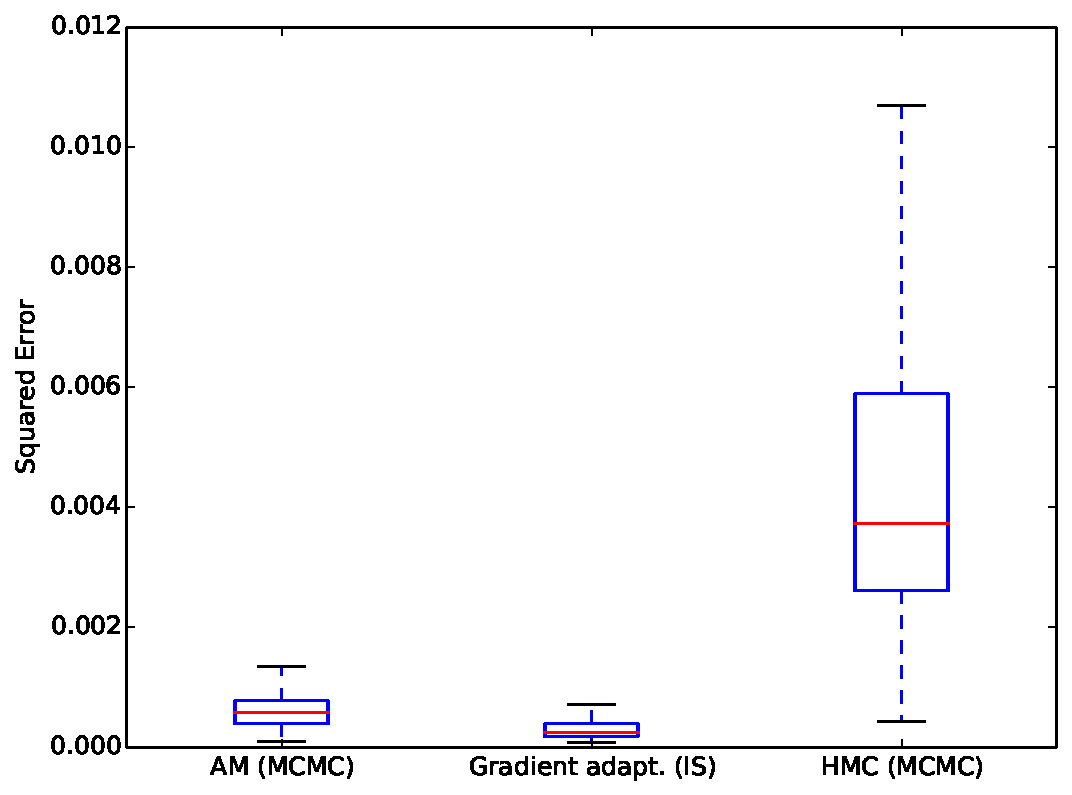
\includegraphics[width=0.8\textwidth]{figures/gpmc_Credit_boxplot.pdf} 
\caption{Logistic regression: Squared errors of mean estimate averaged across dimensions. Algorithms not shown are widely off scale.}
\label{fig:cred_worst}
\end{minipage}\hfill
\begin{minipage}[t]{0.5\textwidth}
\centering
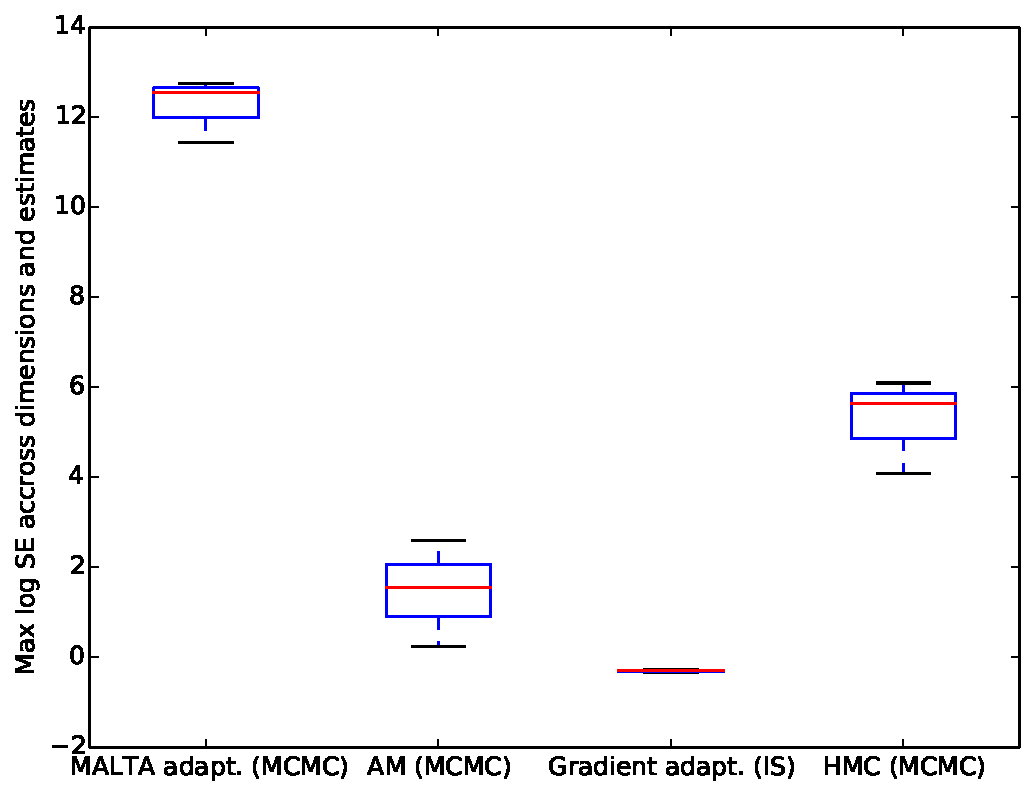
\includegraphics[width=0.75\textwidth]{figures/Credit_worst.pdf} 
\caption{Logistic regression: Maximum log SE across estimates of posterior variance and mean and across dimensions.} 

\label{fig:cred_worst}
\end{minipage}

\end{center}
\end{figure}

\subsection{Evidence Estimation}
Evidence estimates using GRIS quickly stabilized. I assesed MSE of evidence estimates for the $t$-Mixture target and the Logistic Regression model  (Figure \ref{fig:ev}). The log evidences where $-1000$ and $-504$, respectively.

\begin{figure}[tbp]
\begin{center}
\centering
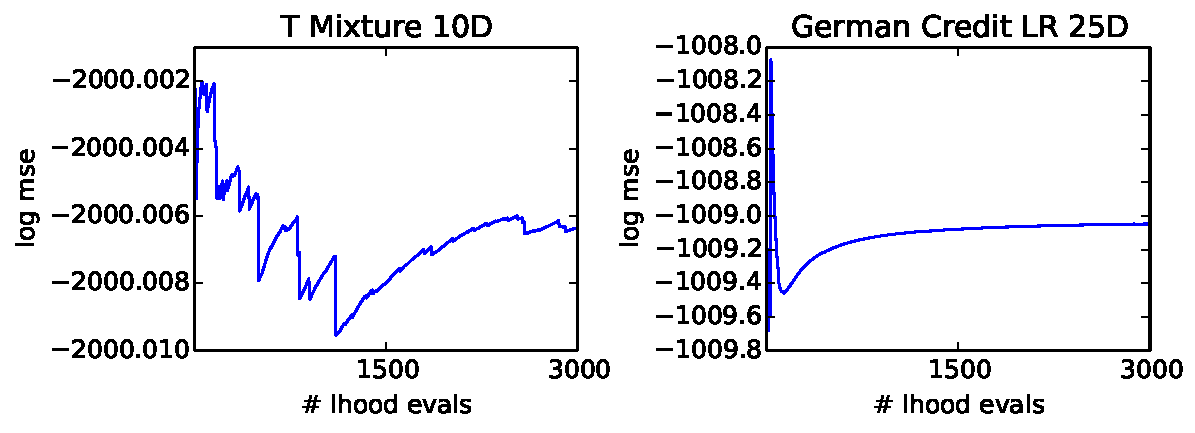
\includegraphics[width=0.8\textwidth]{figures/evidence_mse_plot.pdf} 
\caption{Evidence estimates}
\label{fig:ev}

\end{center}
\end{figure}


\section{Conclusions}
In this paper, I presented Gradient IS, a variant of Sequential Monte Carlo. The algorithm uses gradient information and  a covariance matrix adapted to collected posterior samples to construct a multivariate normal proposal distribution for SMC with static target distributions. GRIS was shown to give very good performance in posterior sampling and provide stable estimates for the normalizing constant of the target distribution (also known as model evidence).

%\input{Chapters/Chapter2} 
%\input{Chapters/Chapter3}
%\input{Chapters/Chapter4} 
%\input{Chapters/Chapter5} 
%\input{Chapters/Chapter6} 
%\input{Chapters/Chapter7} 

%----------------------------------------------------------------------------------------
%	THESIS CONTENT - APPENDICES
%----------------------------------------------------------------------------------------

\addtocontents{toc}{\vspace{2em}} % Add a gap in the Contents, for aesthetics

\appendix % Cue to tell LaTeX that the following 'chapters' are Appendices

% Include the appendices of the thesis as separate files from the Appendices folder
% Uncomment the lines as you write the Appendices

\chapter{Fundamental Monte Carlo Algorithms}

\section{Fundamental MCMC algorithms}

\subsection{Langevin Monte Carlo}
\label{sec:lmc}
Metropolis Adjusted Langevin Truncated Algorithm (MALTA) \cite{Roberts1996} and Hamiltonian Monte Carlo (HMC) \cite{Neal2011} are two well known sampling algorithms that make use of gradient information. In the following, we will denote the target density as $f$. Often times, this will we the posterior of a Bayesian model which can be evaluated only proportionally by multiplying the prior and likelihood at a given a point. \\
 HMC is probably better known in the Machine Learning community, but it is notoriously complex and its description is beyond the scope of this pape. For a thorough introduction see e.g. \cite{Neal2011,Bishop2007}. The special case of HMC however, MALTA, is closely related to the algorithm proposed in this paper and a concise introduction will be given. MALTA is a variant of the Metropolis-Hastings MCMC algorithm where, given the current state of the Markov Chain $\smp'$, a proposal for a new state $\smp$ is sampled from the multivariate normal density
$$q(\cdot | \smp') = N(\cdot | \smp'  + D(\nabla~\textrm{log}~f(\smp' )), C)$$
where $D$ is a drift function. For consistency reasons, the MALTA variant 
used in the evaluation section will use $D(\nabla~\textrm{log}~f(\smp' )) = \delta\nabla~\textrm{log}~f(\smp')$ for $0 \leq \delta \leq$ 1. The covariance matrix $C$ is fixed by the user prior to running the algorithm.
The proposed new state $\smp$ is then accepted with the usual Metropolis-Hasting acceptance probability $$min\left(1,\frac{f(\smp')q(\smp | \smp')}{f(\smp)q(\smp' | \smp)}\right)$$ and recorded as a sample.
 If the proposed state is rejected, the chain remains at state $\smp'$ (which is recorded as a sample again). The Markov Chain is ergodic with respect to $f$, i.e. the samples produced are approximately from $f$, which is guaranteed by using the Metropolis-Hastings correction. The samples can be used to estimate the expectation $H$ of some function of interest $h$ with respect to the target density $f$ using the law of large numbers as
 $$H = \int h(x) f(x) \textrm{d}x \approx 1/N \sum_{i=1}^Nh(\smp_i)$$
where $\smp_i$ ranges over the samples and $N$ is the number of samples.

\section{Fundamental SMC algorithms}

\subsection{Importance Sampling and SMC}
\label{sec:ismc}
Importance Sampling takes a different approach. Instead of trying to sample approximately from $f$, it samples from some proposal density $q$ instead. Rather than correcting for the change of distribution using Metropolis-Hastings, the Importance Sampling estimator simply weighs each sample $\smp$ by the so called importance weight $w(\smp) = f(\smp)/q(\smp)$. In the case where $f$ is not normalized, which is the usual case when estimating a Bayesian posterior, the self-normalized Importance Sampling estimator for $H$ given by

 $$H = \int h(x) w(x) q(x) \textrm{d}x \approx \frac{1}{\sum_{i=1}^N w(\smp_i)} \sum_{i=1}^N w(\smp_i) h(\smp_i)$$
 
Sequential Monte Carlo (SMC) \cite{Doucet2001a}  builds on Importance Sampling and was originally devised to sample from a sequence of target distributions. For ease of exposition, I will first consider the case where the same target distribution is used at each iteration, a special case known as Population Monte Carlo (PMC). From this, an extension to  sequence of targets is straight forward and given in Section \ref{sec:seqin} for the case of static models (i.e. not time series).
In Population Monte Carlo, we first gather a set of $p$ samples (also called \emph{particles} in SMC) $\smp_1,\dots,\smp_p$ from proposal densities $q_1,\dots,q_p$ which are assigned weights $w(\smp_i)=f(\smp_i)/q_i(\smp_i)$. Instead of using these weighted samples directly with the Importance Sampling estimator to evaluate the integral of interest, we resample  $\smp_1,\dots,\smp_p$ with replacement according to their respective weights, adding the resulting set to a set of unweighted samples $S$. This is called Importance Resampling and produces a sample set that is approximately coming from the posterior \citep{Rubin1987}. Several methods exist for this step, the easiest being multinomial resampling. See \cite{Douc2005} for a review including some theoretical results. 
Previous samples can now be used to construct proposal distributions for the next iteration.
In the simplest case this could be centering a proposal distribution on a previous sample. The procedure is iterated until $S$ is deemed large enough. The integral of interest can now simply be computed by
$$H = \int h(x) f(x) \textrm{d}x \approx 1/|S| \sum_{\smp \in S}^Nh(\smp)$$
Moreover, the marginal likelihood $Z$ of the data (also called evidence of the model or normalizing constant of $f$) can be approximated by the formula
$$Z \approx 1/N_w \sum_{i=1}^{N_w} w_i$$
where $w_i$ are the weights that have been gathered from the stage before resampling and $N_w$ is the total number of weights.

A major argument for Gradient IS is the ability to approximate the marginal likelihood \emph{and} the target distribution as good as or better than previous gradient-informed and/or adaptive sampling algorithms while being extremely simple to implement. For example, this opens the possibility to routinely compute Bayes factors (and thus do Bayesian Model selection) as a by-product of very  efficient posterior sampling instead of using special inference techniques geared towards only computing $Z$.

%\input{Appendices/AppendixB}
%\input{Appendices/AppendixC}

\addtocontents{toc}{\vspace{2em}} % Add a gap in the Contents, for aesthetics

\backmatter

%----------------------------------------------------------------------------------------
%	BIBLIOGRAPHY
%----------------------------------------------------------------------------------------

\label{Bibliography}

\lhead{\emph{Bibliography}} % Change the page header to say "Bibliography"

\bibliographystyle{apalike} % Use the "unsrtnat" BibTeX style for formatting the Bibliography

\bibliography{Bibliography} % The references (bibliography) information are stored in the file named "Bibliography.bib"

\end{document}  